\subsubsection{Rotationsmatricer}
\label{sec:rot_matricer}
Hvis vi vil rotere et punkt eller en vektor omkring nul-punktet i et koordinatsystem kan vi bruge en rotationsmatrix \cite{rotationsmatricer}.
En rotationsmatrix er en matrix der, hvis multipliceret sammen med en anden matrix, roterer en vektor eller et punkt i et koordinatsystem.
\begin{align}\label{eu_eqn}
  R_x(\theta) = 
  \begin{bmatrix}
    1 & 0 & 0\\ 
    0 & cos \theta & - sin \theta\\ 
    0 & sin \theta & cos \theta
  \end{bmatrix}\\
    R_y(\theta) =
  \begin{bmatrix}
    cos \theta  & 0 & sin \theta\\ 
    0           & 1 & 0\\ 
    -sin \theta & 0 & cos \theta
  \end{bmatrix}\\
    R_z(\theta) = 
  \begin{bmatrix}
    cos \theta & - sin \theta & 0\\ 
    sin \theta & cos \theta & 0\\
    0 & 0 & 1
  \end{bmatrix}
\end{align}
Vi indsætter den vinkel som vi vil drejse vektoren med i radianer og multiplicerer dem sammen som angivet i formlen. Vektoren bliver drejet omkring nul-punktet med netop den mængde radianer som er angivet.
Nedenstående eksempel illustrerer princippet ved at dreje en vektor i rummet.

\begin{equation}
  U=
  \begin{bmatrix}
    0 & 1 & 5
  \end{bmatrix}
\end{equation}
og rotationsvektor \begin{math}R_x\end{math}
\begin{equation}
  R_x(\theta) = 
  \begin{bmatrix}
    1 & 0 & 0\\ 
    0 & cos \theta & - sin \theta\\ 
    0 & sin \theta & cos \theta
  \end{bmatrix}
\end{equation}
Vi tager matrix-vektor-produktet af dem, og indsætter 1 Radian i $R_x$:
\begin{align}
  0*0+1*0+5*0&=0\\
  0*0+1*cos(1)+5*sin(1)&=4.75\\
  0*0+1*(-sin(1))+5*cos(1)&=1.86
\end{align}
Og kalder det for vektor V og indsætter både U og V i nedenstående skitse.
\begin{figure}[H]
  \center
  \begin{tikzpicture}
    \coordinate (O) at (0,0) ;
    \coordinate (u) at (1, 5) ;
    \coordinate (v) at (4.75, 1.86) ;

    \draw[step=1cm,gray,very thin] (-1.9,-1.9) grid (5.9,5.9);
    \foreach \x in {0,1,2,3,4}
      \draw (\x cm,1pt) -- (\x cm,-1pt) node[anchor=north] {$\x$};
    \foreach \y in {0,1,2,3,4}
      \draw (1pt,\y cm) -- (-1pt,\y cm) node[anchor=east] {$\y$};
    \draw[thick,->] (O) -- (4.5,0);
    \draw[thick,->] (O) -- (0,4.5);
    \draw[thick,->] (O) -- (4.5,0) node[anchor=north west] {x};
    \draw[thick,->] (O) -- (0,4.5) node[anchor=south east] {y};

    \draw [blue!50, thick, -{Stealth[width=3mm, length=3mm]}] (O) -- (u);
    \draw [blue!50, thick, -{Stealth[width=3mm, length=3mm]}] (O) -- (v);
    \node [below right] at (u) {$u$};
    \node [below] at (v) {$v$};
    \draw (1, 0.4) arc (10:77:1);
    \node[] at (1,1.2)  {$\theta = 1$};
  \end{tikzpicture}
  % 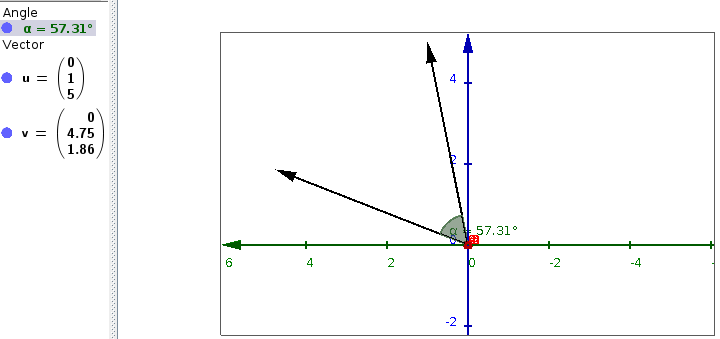
\includegraphics[width=12cm]{rotationsmatrix_eksempel.png}
  \caption{Eksempel på en rotationsmatrix}
  \label{fig:rotationsmatrix_eksempel}
\end{figure}
% Geogebra udregner vinkler i grader, så vi omregner grader til radianer ved hjælp af ligningen:
% \begin{equation}
  % R=d/2*\pi/360=57,31/2*\pi/360\approx1
% \end{equation}
Vi ser at vektor $U$ blev drejet 1 radian, som forventet.
